\chapter{Seven Ways to Make a Full-Time Income While Traveling}

This chapter follows a School of Hard Knocks entrepreneurship lesson curated by LazyingArt LLC. The speaker begins from a blunt contrast: money can come back, but time cannot. The lecture then asks how income can be arranged so that travel is not postponed until after a conventional career has already fixed a person in one place. The answer is not a single formula. It is a sequence of seven mechanisms: remote skill work, travel-embedded employment, product margin, audience monetization, agency packaging, language demand, and institutional sales.

\section{Travel, Time, and the Income Question}

The opening motivation is simple enough to be useful. If time is the scarce resource, then the business question is not merely how to make money. It is how to make money under a constraint of movement. We want income that is not completely tied to one city, one office, or one local employer.

Let \(I\) denote income and \(L\) denote location. A fixed-location arrangement has a strong dependence
\begin{equation}
I = I(L),
\end{equation}
where earning power is attached to a particular place. The lecture is looking for arrangements closer to
\begin{equation}
I \approx I(\text{skill},\text{offer},\text{market}),
\end{equation}
where location still matters, but it is no longer the whole engine of income.

That is the question driving the list: what can we sell, join, package, or represent so that income can continue while we move?

\section{Freelancing: Turning a Skill into a Remote Offer}

The first path is freelancing online. The speaker names Fiverr and Upwork, but the platforms are not the core idea. They are examples of a broader marketplace structure: someone has a problem, someone else has a skill, and the work can be delivered without sharing a physical location.

The lecture moves quickly through the skill inventory: writing, graphic design, editing photography, editing YouTube videos, editing TikToks, managing social media, running Google or Facebook ads, creating content, and producing static posts. These examples should not be flattened into one generic phrase. Their variety is the point. A portable offer can be built from many different skills.

The common structure is
\begin{equation}
\text{remote service}
=
\text{skill}
+
\text{client demand}
+
\text{digital delivery}.
\end{equation}

Freelancing comes first because it is the smallest commercial unit in the lecture. Before we need a brand, audience, agency, or employer relocation package, we need to see that a skill can be sold to a buyer who already wants the result.

\begin{figure}
\centering
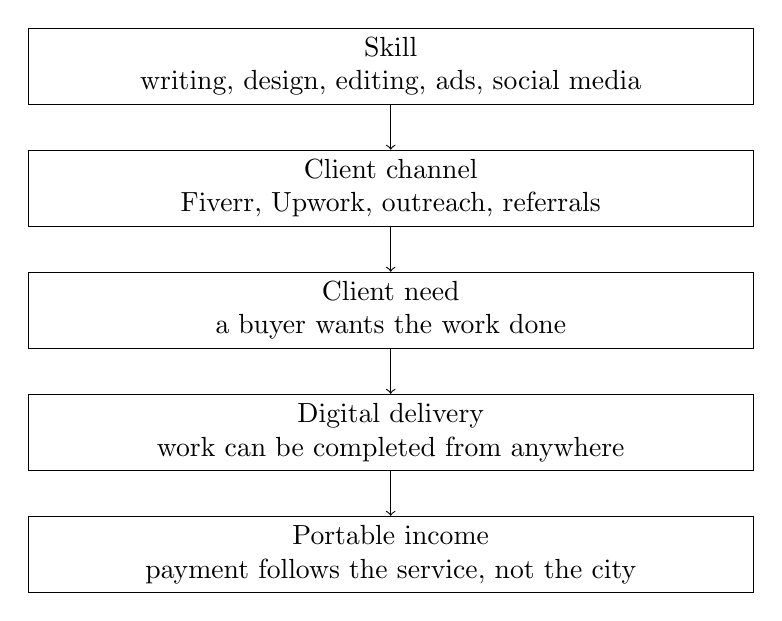
\begin{tikzpicture}
\node[draw, align=center, text width=0.74\linewidth] (skill) at (0,0) {Skill\\writing, design, editing, ads, social media};
\node[draw, align=center, text width=0.74\linewidth] (channel) at (0,-1.55) {Client channel\\Fiverr, Upwork, outreach, referrals};
\node[draw, align=center, text width=0.74\linewidth] (need) at (0,-3.10) {Client need\\a buyer wants the work done};
\node[draw, align=center, text width=0.74\linewidth] (delivery) at (0,-4.65) {Digital delivery\\work can be completed from anywhere};
\node[draw, align=center, text width=0.74\linewidth] (income) at (0,-6.20) {Portable income\\payment follows the service, not the city};
\draw[->] (skill) -- (channel);
\draw[->] (channel) -- (need);
\draw[->] (need) -- (delivery);
\draw[->] (delivery) -- (income);
\end{tikzpicture}
\end{figure}

\section{Hospitality: Working Inside the Travel System}

The second path changes the model. Freelancing uses the internet to carry work across distance. Hospitality uses an industry that already moves people through distance. The speaker names cruise ships, yacht crews, flight attendants, resorts, and international hotels.

Here the worker is not fully location-independent in the freelancer's sense. Instead, movement is built into the job:
\begin{equation}
\text{travel}
\subset
\text{employment conditions}.
\end{equation}

The examples are deliberately concrete. A yacht or cruise ship may move from Miami toward the Virgin Islands. A flight attendant may reach Europe through international routes. A resort or hotel can place the worker in the Bahamas, including the speaker's example of Atlantis, or in another island or country.

The mechanism is access. The worker does not yet own the business system. But if an industry needs labor in the places people want to go, then the job itself can pay part of the travel cost, provide movement, or attach work to a desired location. This broadens the lecture: portable income is not only laptop income.

\section{E-Commerce: Unit Margin and Distribution}

The third path is starting an e-commerce brand. This is where the lecture gives its clearest arithmetic. The speaker's example is t-shirts: find a manufacturer, buy or produce a product for roughly five, ten, or fifteen dollars, and sell it for roughly twenty, twenty-five, or thirty dollars. The transcript is garbled at one point, but the intended sequence is best read cautiously as \(20\), \(25\), and \(30\) dollars.

Let \(C\) be unit cost and \(P\) be sale price:
\begin{align}
C &\in \{\$5,\ \$10,\ \$15\},\\
P &\in \{\$20,\ \$25,\ \$30\}.
\end{align}
The gross profit per unit is then
\begin{equation}
\pi = P-C.
\end{equation}

When the speaker says this creates a return on investment, we can write the simplest unit-level reconstruction as
\begin{equation}
\mathrm{ROI}=\frac{P-C}{C}.
\end{equation}
This is a deliberately narrow formula. It does not include advertising cost, shipping, fulfillment, platform fees, refunds, taxes, or labor. It only captures the spread between what the product costs and what the customer pays.

\subsection{Question \& Answer}

\paragraph{Question.}
What makes this more than buying low and selling high?

\paragraph{Answer.}
The lecture answers by immediately widening the example. The t-shirt arithmetic is only the starting point. A brand also needs a product choice, a supplier or manufacturer, possibly a designer, a storefront such as Shopify, and distribution through Google, Facebook, TikTok, Instagram, branded content, or viral content. Margin tells us that a transaction can work. Distribution tells us whether the transaction can repeat.

\subsection{A Worked Unit Example}

Suppose a shirt costs
\begin{equation}
C=\$10
\end{equation}
and sells for
\begin{equation}
P=\$25.
\end{equation}
Then the gross profit per unit is
\begin{align}
\pi &= P-C\\
&= \$25-\$10\\
&= \$15.
\end{align}
The simple unit-level return is
\begin{align}
\mathrm{ROI}
&= \frac{P-C}{C}\\
&= \frac{15}{10}\\
&= 1.5.
\end{align}
So before omitted costs, the unit shows a \(150\%\) return on the unit cost. The lecture's implied discipline is that this arithmetic is not enough by itself. A product margin becomes a business only if supply, storefront, and marketing work together.

\begin{figure}
\centering
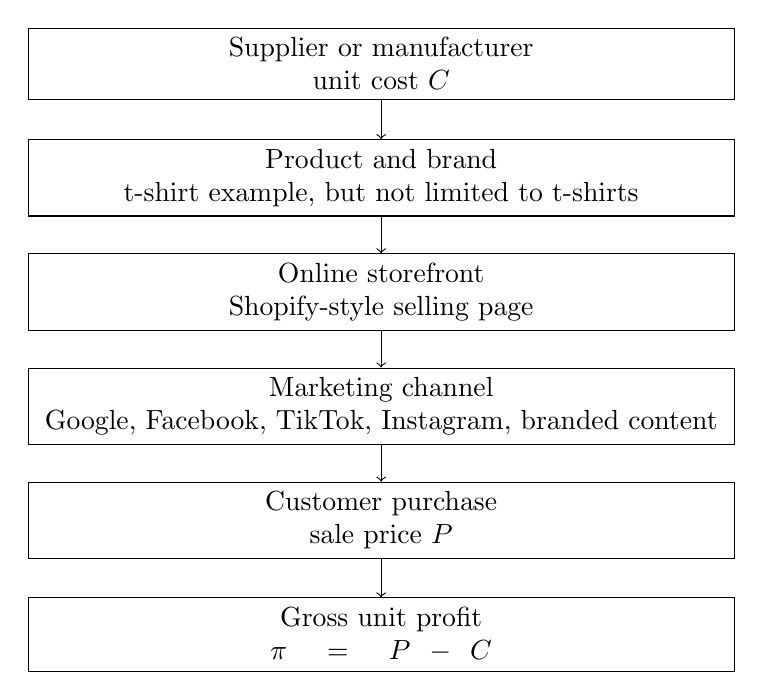
\begin{tikzpicture}
\node[draw, align=center, text width=0.72\linewidth] (source) at (0,0) {Supplier or manufacturer\\unit cost \(C\)};
\node[draw, align=center, text width=0.72\linewidth] (product) at (0,-1.45) {Product and brand\\t-shirt example, but not limited to t-shirts};
\node[draw, align=center, text width=0.72\linewidth] (store) at (0,-2.90) {Online storefront\\Shopify-style selling page};
\node[draw, align=center, text width=0.72\linewidth] (market) at (0,-4.35) {Marketing channel\\Google, Facebook, TikTok, Instagram, branded content};
\node[draw, align=center, text width=0.72\linewidth] (sale) at (0,-5.80) {Customer purchase\\sale price \(P\)};
\node[draw, align=center, text width=0.72\linewidth] (profit) at (0,-7.25) {Gross unit profit\\\(\pi=P-C\)};
\draw[->] (source) -- (product);
\draw[->] (product) -- (store);
\draw[->] (store) -- (market);
\draw[->] (market) -- (sale);
\draw[->] (sale) -- (profit);
\end{tikzpicture}
\end{figure}

The speaker then says that it does not have to be t-shirts. That transition matters. The lesson is not a shirt business. The lesson is a structure: find a product, find a supply path, put it in front of buyers, and keep enough spread to survive the costs of selling.

\section{Content Creation: Audience Before Travel Income}

The fourth path is content creation. The speaker calls it one of the most fun ways to get paid to travel, but immediately introduces a caution. If someone leaves with little money and no audience, hoping to start fresh on an island or in a new country, there is a real chance of running out of money quickly.

That warning is the center of the section. The income mechanism is not travel plus a camera. It is attention converted into offers:
\begin{equation}
\text{creator income}
=
f(\text{audience},\text{trust},\text{content},\text{brand demand}).
\end{equation}

\subsection{Question \& Answer}

\paragraph{Question.}
Can we build the audience after we arrive?

\paragraph{Answer.}
The lecture's answer is cautious: build the base first. Travel can provide material, but the audience is the asset that makes the material commercially useful. Brands have a reason to pay only when there is already attention, trust, and proof that the creator can move people toward a product or service.

The speaker lists several ways a creator can earn: affiliate deals, selling one's own products, merchandise, launching an e-commerce brand, travel blogging, working with brands, and becoming a brand ambassador. If an affiliate is paid a rate \(r\) on referred sales \(S_{\mathrm{referred}}\), a simple reconstruction is
\begin{equation}
I_{\mathrm{affiliate}}=rS_{\mathrm{referred}}.
\end{equation}
This is not a displayed lecture equation; it is a compact way to express the speaker's phrase about taking a percentage of sales.

The lecture also gives a concrete claim: some long-term ambassador programs may pay
\begin{equation}
A \approx \$10{,}000\text{--}\$20{,}000
\end{equation}
for a series of paid advertisements. In the final reading, this should remain a claim about some programs, not a promised rate for all creators.

\section{Agencies: Packaging Skill into a Client System}

The fifth path is starting an agency. This returns us to skills, but at a higher level of packaging. A freelancer sells a task. An agency sells a repeatable capability to brands or companies.

The transcript names photography, digital marketing, social media growth, programming, and written software for companies. These are not random examples; they are skills that can be bundled into a service offer:
\begin{equation}
\text{agency offer}
=
\text{skill}
+
\text{packaging}
+
\text{client value}.
\end{equation}

The lecturer also makes a practical distinction. Some agency work requires physical presence. If a company needs content shot on location, then the worker may need to be there. But if the work is content strategy, programming, software, or remote marketing execution, then the service can be delivered from a distance.

That distinction keeps the section grounded. The question is not whether the service sounds modern or impressive. The question is whether the promised value survives remote delivery.

\section{Language Tuition and Sales: Demand from Institutions}

The sixth path is language tuition. The speaker describes teaching English in a foreign country where English instruction is in demand. The point is not merely that a language skill can be monetized. The point is that some education markets may be organized enough to pay income, relocation, and housing support.

The mechanism can be written as
\begin{equation}
\text{teaching income}
=
\text{English ability}
+
\text{local demand}
+
\text{institutional placement}.
\end{equation}
The lecture names children, adults, schools, and teachers as possible learners or settings. The portable asset is English fluency, but the demand comes from a local market that needs that fluency taught.

The seventh path is sales representation. The speaker names information technology, defense, insurance, and pharmaceutical industries. These industries need people who can sell products or services to other companies. In this case, the traveler does not necessarily own the product. The portable asset is sales competence: persuasion, follow-up, relationship management, and closing.

The transcript includes the claim that some large industries may pay
\begin{equation}
S>\$100{,}000
\end{equation}
annually to people who do strong sales work on the road. This is best written as an upper-end possibility in some industries, not as a guarantee. The lecture's mechanism is high-ticket institutional selling: when the product or service is valuable enough, the organization can afford to pay well for someone who produces revenue.

\section{The Seven Mechanisms Together}

The lecture is presented as a list, but the list has an internal order. It begins with individual skill, moves to travel-embedded employment, then to product and audience systems, and finally to institutional demand.

\begin{figure}
\centering
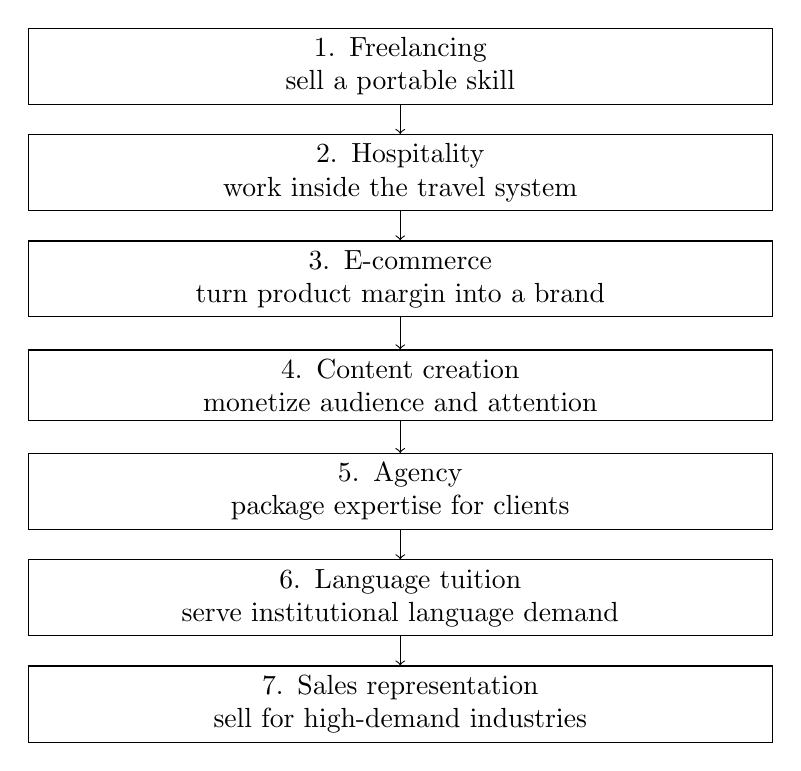
\begin{tikzpicture}
\node[draw, align=center, text width=0.76\linewidth] (a) at (0,0) {1. Freelancing\\sell a portable skill};
\node[draw, align=center, text width=0.76\linewidth] (b) at (0,-1.35) {2. Hospitality\\work inside the travel system};
\node[draw, align=center, text width=0.76\linewidth] (c) at (0,-2.70) {3. E-commerce\\turn product margin into a brand};
\node[draw, align=center, text width=0.76\linewidth] (d) at (0,-4.05) {4. Content creation\\monetize audience and attention};
\node[draw, align=center, text width=0.76\linewidth] (e) at (0,-5.40) {5. Agency\\package expertise for clients};
\node[draw, align=center, text width=0.76\linewidth] (f) at (0,-6.75) {6. Language tuition\\serve institutional language demand};
\node[draw, align=center, text width=0.76\linewidth] (g) at (0,-8.10) {7. Sales representation\\sell for high-demand industries};
\draw[->] (a) -- (b);
\draw[->] (b) -- (c);
\draw[->] (c) -- (d);
\draw[->] (d) -- (e);
\draw[->] (e) -- (f);
\draw[->] (f) -- (g);
\end{tikzpicture}
\end{figure}

We can also classify the seven paths by the economic asset being used.

\begin{table}
\centering
\begin{tabular}{l l}
Path & Main economic asset \\
Freelancing & Remote skill sold to clients \\
Hospitality & Job access inside travel industries \\
E-commerce & Product margin plus distribution \\
Content creation & Audience and brand attention \\
Agency & Packaged expertise for companies \\
Language tuition & English ability and relocation demand \\
Sales representation & Sales skill in large industries \\
\end{tabular}
\end{table}

This classification is useful because it prevents the list from becoming a motivational blur. Each path asks for a different asset. If we know which asset we actually have, we can ask a sharper question about which market will pay for it.

\section{Summary}

The lecture's promise is not that every path is equally easy, equally profitable, or equally reliable. Its stronger claim is structural: location freedom can come from different kinds of commercial design. We can sell a skill remotely, join work that already moves, build product margin, monetize an audience, package expertise for clients, teach where language demand is strong, or sell for institutions that pay for revenue.

The mathematics is modest because the source material is practical rather than formal. Still, the arithmetic clarifies the mechanisms. In e-commerce, \(P-C\) is the beginning of the business, not the whole business. In creator work, an affiliate percentage matters only if there is referred demand. In sales, a six-figure compensation claim depends on industry demand and a person's ability to produce revenue on the road.

The final lesson is commercial rather than sentimental. Travel becomes more feasible when income is attached to a portable asset. The asset may be a skill, a product, an audience, an agency package, a language ability, or a sales capacity. The work is to identify the asset honestly, then match it to a market that can pay while we move.